\documentclass[11pt, a4j, dvipdfmx]{jarticle}
\usepackage{docmute}  % 上手く分割するために必要
\usepackage{amsmath}
\usepackage{setspace}
\usepackage{mathtools}
\usepackage[dvipdfmx]{graphicx}  % Include figure files
% \usepackage[varg]{txfonts}
\usepackage{bm}  % bold math
\usepackage{here}
\usepackage{array}
\usepackage[T1]{fontenc}
\usepackage{etoolbox}
\usepackage[top=30truemm,bottom=30truemm,left=25truemm,right=25truemm]{geometry}  % 余白
\usepackage{comment}
\usepackage{cases}
\usepackage[version=3]{mhchem}
\usepackage{layout}
\usepackage{wrapfig}
\usepackage{indentfirst}
\usepackage{txfonts}


%\renewcommand{\indent}{\hspace*{1zw}}
\renewcommand{\abstractname}{}
\renewcommand{\figurename}{Fig.}
\renewcommand{\thefootnote}{\fnsymbol{footnote}}
\renewcommand{\thesection}{\arabic{section}}


\pagestyle{plain}
%%%%%%%%%%%%%%%%%%%%%%%%%%%%%%%%%%%%%%%%%%%%%%%%%%%%%%%%%%%%%%%%%%%%%%%%%%
\makeatletter%% プリアンブルで定義する場合は必須
\patchcmd{\maketitle}{\@fnsymbol}{\@alph}{}{}  % Footnote numbers from symbols to small letters
\long\def\@makecaption#1#2{% \@makecaption を再定義します
  \vskip\abovecaptionskip
  \iftdir\sbox\@tempboxa{#1\hskip1zw#2}%
    \else\sbox\@tempboxa{#1~ #2}  % ここの : を ~ に変更する
  \fi
  \ifdim \wd\@tempboxa >\hsize% 
    \iftdir #1\hskip1zw#2\relax\par
      \else #1~ #2\relax\par\fi  % ここの : を ~ に変更する
  \else
    \global \@minipagefalse
    \hbox to\hsize{\hfil\box\@tempboxa\hfil}  % センタリング
%   \hbox to\hsize{\box\@tempboxa\hfil}%      左詰め
%   \hbox to\hsize{\hfil\box\@tempboxa}%      右詰め
  \fi
  \vskip\belowcaptionskip}
 \DeclareRobustCommand\cite{\unskip
\@ifnextchar[{\@tempswatrue\@citex}{\@tempswafalse\@citex[]}}
 \def\@cite#1#2{$^{[\hbox{\scriptsize{#1\if@tempswa , #2\fi}]}}$}
 \def\@biblabel#1{[#1]}
\makeatother%% プリアンブルで定義する場合は必須

\setlength{\columnsep}{8  truemm}
\setlength{\linewidth}{90 truemm}
  % usepackage, renewcommand, macroなど

\begin{document}

\documentclass[12pt, a4j, dvipdfmx]{jarticle}
\usepackage{amsmath}
\usepackage{setspace}
\usepackage{mathtools}
\usepackage[dvipdfmx]{graphicx}  % Include figure files
% \usepackage[varg]{txfonts}
\usepackage{bm}  % bold math
\usepackage{here}
\usepackage{array}
\usepackage[T1]{fontenc}
\usepackage{etoolbox}
\usepackage[top=30truemm,bottom=30truemm,left=25truemm,right=25truemm]{geometry}  % 余白
\usepackage{comment}
\usepackage{cases}
\usepackage[version=3]{mhchem}
\usepackage{layout}
\usepackage{wrapfig}
\usepackage{indentfirst}
\usepackage{txfonts}


%\renewcommand{\indent}{\hspace*{1zw}}
\renewcommand{\abstractname}{}
\renewcommand{\figurename}{Fig.}
\renewcommand{\thefootnote}{\fnsymbol{footnote}}
\renewcommand{\thesection}{\arabic{section}}


\pagestyle{plain}
%%%%%%%%%%%%%%%%%%%%%%%%%%%%%%%%%%%%%%%%%%%%%%%%%%%%%%%%%%%%%%%%%%%%%%%%%%
\makeatletter%% プリアンブルで定義する場合は必須
\patchcmd{\maketitle}{\@fnsymbol}{\@alph}{}{}  % Footnote numbers from symbols to small letters
\long\def\@makecaption#1#2{% \@makecaption を再定義します
  \vskip\abovecaptionskip
  \iftdir\sbox\@tempboxa{#1\hskip1zw#2}%
    \else\sbox\@tempboxa{#1~ #2}  % ここの : を ~ に変更する
  \fi
  \ifdim \wd\@tempboxa >\hsize% 
    \iftdir #1\hskip1zw#2\relax\par
      \else #1~ #2\relax\par\fi  % ここの : を ~ に変更する
  \else
    \global \@minipagefalse
    \hbox to\hsize{\hfil\box\@tempboxa\hfil}  % センタリング
%   \hbox to\hsize{\box\@tempboxa\hfil}%      左詰め
%   \hbox to\hsize{\hfil\box\@tempboxa}%      右詰め
  \fi
  \vskip\belowcaptionskip}
 \DeclareRobustCommand\cite{\unskip
\@ifnextchar[{\@tempswatrue\@citex}{\@tempswafalse\@citex[]}}
 \def\@cite#1#2{$^{[\hbox{\scriptsize{#1\if@tempswa , #2\fi}]}}$}
 \def\@biblabel#1{[#1]}
\makeatother%% プリアンブルで定義する場合は必須

\setlength{\columnsep}{8  truemm}
\setlength{\linewidth}{90 truemm}


\begin{document}


\begin{titlepage}
    \begin{center}
        \vspace*{50truept}
        {\huge 卒業論文 (2020年)} \\
        \vspace*{100truept}
        {\huge \textbf{せん断流下における\\マイクロスイマー希薄分散系の動的挙動}} \\
        \vspace{120truept}
        {\LARGE 京都大学工学部工業化学科} \\
        {\LARGE 化学プロセス工学コース} \\
        {\LARGE 移動現象論分野} \\
        \vspace{50truept}
        {\LARGE 荊尾\ 太雅} \\
        \vspace{50truept}
    \end{center}
\end{titlepage}


\end{document}
  % タイトル
\documentclass[12pt, a4j, dvipdfmx]{jarticle}
\usepackage{amsmath}
\usepackage{setspace}
\usepackage{mathtools}
\usepackage[dvipdfmx]{graphicx}  % Include figure files
% \usepackage[varg]{txfonts}
\usepackage{bm}  % bold math
\usepackage{here}
\usepackage{array}
\usepackage[T1]{fontenc}
\usepackage{etoolbox}
\usepackage[top=30truemm,bottom=30truemm,left=25truemm,right=25truemm]{geometry}  % 余白
\usepackage{comment}
\usepackage{cases}
\usepackage[version=3]{mhchem}
\usepackage{layout}
\usepackage{wrapfig}
\usepackage{indentfirst}
\usepackage{txfonts}


%\renewcommand{\indent}{\hspace*{1zw}}
\renewcommand{\abstractname}{}
\renewcommand{\figurename}{Fig.}
\renewcommand{\thefootnote}{\fnsymbol{footnote}}
\renewcommand{\thesection}{\arabic{section}}


\pagestyle{plain}
%%%%%%%%%%%%%%%%%%%%%%%%%%%%%%%%%%%%%%%%%%%%%%%%%%%%%%%%%%%%%%%%%%%%%%%%%%
\makeatletter%% プリアンブルで定義する場合は必須
\patchcmd{\maketitle}{\@fnsymbol}{\@alph}{}{}  % Footnote numbers from symbols to small letters
\long\def\@makecaption#1#2{% \@makecaption を再定義します
  \vskip\abovecaptionskip
  \iftdir\sbox\@tempboxa{#1\hskip1zw#2}%
    \else\sbox\@tempboxa{#1~ #2}  % ここの : を ~ に変更する
  \fi
  \ifdim \wd\@tempboxa >\hsize% 
    \iftdir #1\hskip1zw#2\relax\par
      \else #1~ #2\relax\par\fi  % ここの : を ~ に変更する
  \else
    \global \@minipagefalse
    \hbox to\hsize{\hfil\box\@tempboxa\hfil}  % センタリング
%   \hbox to\hsize{\box\@tempboxa\hfil}%      左詰め
%   \hbox to\hsize{\hfil\box\@tempboxa}%      右詰め
  \fi
  \vskip\belowcaptionskip}
 \DeclareRobustCommand\cite{\unskip
\@ifnextchar[{\@tempswatrue\@citex}{\@tempswafalse\@citex[]}}
 \def\@cite#1#2{$^{[\hbox{\scriptsize{#1\if@tempswa , #2\fi}]}}$}
 \def\@biblabel#1{[#1]}
\makeatother%% プリアンブルで定義する場合は必須

\setlength{\columnsep}{8  truemm}
\setlength{\linewidth}{90 truemm}


\begin{document}


\setcounter{tocdepth}{3}  % 目次の深さ
\tableofcontents


\end{document}
  % 目次

\newpage
\documentclass[11pt, a4j, dvipdfmx]{jarticle}
\usepackage{amsmath}
\usepackage{setspace}
\usepackage{mathtools}
\usepackage[dvipdfmx]{graphicx}  % Include figure files
% \usepackage[varg]{txfonts}
\usepackage{bm}  % bold math
\usepackage{here}
\usepackage{array}
\usepackage[T1]{fontenc}
\usepackage{etoolbox}
\usepackage[top=30truemm,bottom=30truemm,left=25truemm,right=25truemm]{geometry}  % 余白
\usepackage{comment}
\usepackage{cases}
\usepackage[version=3]{mhchem}
\usepackage{layout}
\usepackage{wrapfig}
\usepackage{indentfirst}
\usepackage{txfonts}


%\renewcommand{\indent}{\hspace*{1zw}}
\renewcommand{\abstractname}{}
\renewcommand{\figurename}{Fig.}
\renewcommand{\thefootnote}{\fnsymbol{footnote}}
\renewcommand{\thesection}{\arabic{section}}


\pagestyle{plain}
%%%%%%%%%%%%%%%%%%%%%%%%%%%%%%%%%%%%%%%%%%%%%%%%%%%%%%%%%%%%%%%%%%%%%%%%%%
\makeatletter%% プリアンブルで定義する場合は必須
\patchcmd{\maketitle}{\@fnsymbol}{\@alph}{}{}  % Footnote numbers from symbols to small letters
\long\def\@makecaption#1#2{% \@makecaption を再定義します
  \vskip\abovecaptionskip
  \iftdir\sbox\@tempboxa{#1\hskip1zw#2}%
    \else\sbox\@tempboxa{#1~ #2}  % ここの : を ~ に変更する
  \fi
  \ifdim \wd\@tempboxa >\hsize% 
    \iftdir #1\hskip1zw#2\relax\par
      \else #1~ #2\relax\par\fi  % ここの : を ~ に変更する
  \else
    \global \@minipagefalse
    \hbox to\hsize{\hfil\box\@tempboxa\hfil}  % センタリング
%   \hbox to\hsize{\box\@tempboxa\hfil}%      左詰め
%   \hbox to\hsize{\hfil\box\@tempboxa}%      右詰め
  \fi
  \vskip\belowcaptionskip}
 \DeclareRobustCommand\cite{\unskip
\@ifnextchar[{\@tempswatrue\@citex}{\@tempswafalse\@citex[]}}
 \def\@cite#1#2{$^{[\hbox{\scriptsize{#1\if@tempswa , #2\fi}]}}$}
 \def\@biblabel#1{[#1]}
\makeatother%% プリアンブルで定義する場合は必須

\setlength{\columnsep}{8  truemm}
\setlength{\linewidth}{90 truemm}


\begin{document}


\section{緒言}
\label{sec:introduction}


\subsection{研究背景}
\par
マイクロスイマーとは,水中の微生物に代表される,周辺流体との流体力学的相互作用により,粘性流体中を自己推進する微小な物体の総称である.
マイクロスイマーが分散した流体は,自己泳動しないコロイド粒子が分散した流体とは,大きく性質が異なることが知られている.
マイクロスイマーの挙動の解析は,医療器具などの汚染の原因となるバイオフィルムの形成過程の説明や,
ドラッグデリバリーシステムへの応用など,様々な分野での活用が期待されている.
しかし,流体的相互作用が複雑であり,莫大な計算コストを要することから,
数値シミュレーションによる解析例が少ない対象でもある.
そのため,マイクロスイマーを解析するには計算負荷を軽減することが重要となる.
    \begin{figure}[htbp]
        \centering
        \includegraphics[scale=0.7]{/Users/taiga/Projects/lab/thesis/components/chapter1/figs/puller.png}
        \caption{マイクロスイマーの一種であるクラミドモナスの泳動の様子\cite{Chlamydomonas}}
    \end{figure}


\subsection{研究目的}
\label{sec:purpose}

\par
マイクロスイマー分散系がコロイド分散系と異なる値を示す一例として有効粘度が挙げられる.
有効粘度は,式\eqref{eq:effective_viscosity}のように表される.
    \begin{equation}
        \eta_\mathrm{eff} = \frac{\sigma}{\dot{\gamma}}
        \label{eq:effective_viscosity}
    \end{equation}
ここで,$\sigma$は系のせん断応力,$\dot{\gamma}$はせん断速度である.
Rafa\"iらは,泳動する通常のクラミドモナスと泳動しない非活性のクラミドモナスの分散系とで,
有効粘度の値に違いが見られることを実験により検証しており,
クラミドモナスの泳動方向が異方的であることから,その値の違いが生じると述べている\cite{effective_viscosity}.
%--
そこで,シミュレーション上でマイクロスイマーの進行方向が異方的になる原因と考えられる性質を付加し,
その挙動を調べることを本研究の目的とした.
%--
マイクロスイマーの進行方向を異方的とする性質や系の状態はいくつか考えられる.
本研究では,球状のマイクロスイマーにおいて,その重心が球の中心から後方にずれているbottom heavy性を持ち,
せん断流下に存在することで異方的挙動を再現できると考え,
それらを考慮したシミュレーションを行った.
また,研究の第一歩として,マイクロスイマー単体が存在する系を考えた.
    \begin{figure}[H]
        \centering
        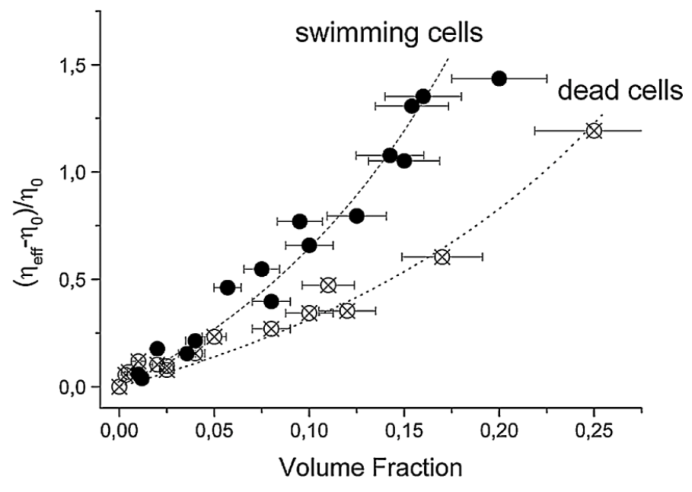
\includegraphics[scale=0.6]{/Users/taiga/Projects/lab/thesis/components/chapter1/figs/previous_research.pdf}
        \caption{泳動するクラミドモナスと泳動しないクラミドモナスの有効粘度\cite{effective_viscosity}.
        黒いプロットが泳動するクラミドモナスの分散系を,白いプロットが泳動しない非活性なクラミドモナスの分散系を表す.
        泳動の有無により,明らかに値が異なることが分かる.}
    \end{figure}

\end{document}
  % 緒言

\newpage
\documentclass[11pt, a4j, dvipdfmx]{jarticle}
\usepackage{amsmath}
\usepackage{setspace}
\usepackage{mathtools}
\usepackage[dvipdfmx]{graphicx}  % Include figure files
% \usepackage[varg]{txfonts}
\usepackage{bm}  % bold math
\usepackage{here}
\usepackage{array}
\usepackage[T1]{fontenc}
\usepackage{etoolbox}
\usepackage[top=30truemm,bottom=30truemm,left=25truemm,right=25truemm]{geometry}  % 余白
\usepackage{comment}
\usepackage{cases}
\usepackage[version=3]{mhchem}
\usepackage{layout}
\usepackage{wrapfig}
\usepackage{indentfirst}
\usepackage{txfonts}


%\renewcommand{\indent}{\hspace*{1zw}}
\renewcommand{\abstractname}{}
\renewcommand{\figurename}{Fig.}
\renewcommand{\thefootnote}{\fnsymbol{footnote}}
\renewcommand{\thesection}{\arabic{section}}


\pagestyle{plain}
%%%%%%%%%%%%%%%%%%%%%%%%%%%%%%%%%%%%%%%%%%%%%%%%%%%%%%%%%%%%%%%%%%%%%%%%%%
\makeatletter%% プリアンブルで定義する場合は必須
\patchcmd{\maketitle}{\@fnsymbol}{\@alph}{}{}  % Footnote numbers from symbols to small letters
\long\def\@makecaption#1#2{% \@makecaption を再定義します
  \vskip\abovecaptionskip
  \iftdir\sbox\@tempboxa{#1\hskip1zw#2}%
    \else\sbox\@tempboxa{#1~ #2}  % ここの : を ~ に変更する
  \fi
  \ifdim \wd\@tempboxa >\hsize% 
    \iftdir #1\hskip1zw#2\relax\par
      \else #1~ #2\relax\par\fi  % ここの : を ~ に変更する
  \else
    \global \@minipagefalse
    \hbox to\hsize{\hfil\box\@tempboxa\hfil}  % センタリング
%   \hbox to\hsize{\box\@tempboxa\hfil}%      左詰め
%   \hbox to\hsize{\hfil\box\@tempboxa}%      右詰め
  \fi
  \vskip\belowcaptionskip}
 \DeclareRobustCommand\cite{\unskip
\@ifnextchar[{\@tempswatrue\@citex}{\@tempswafalse\@citex[]}}
 \def\@cite#1#2{$^{[\hbox{\scriptsize{#1\if@tempswa , #2\fi}]}}$}
 \def\@biblabel#1{[#1]}
\makeatother%% プリアンブルで定義する場合は必須

\setlength{\columnsep}{8  truemm}
\setlength{\linewidth}{90 truemm}


\begin{document}


\section{計算手法}


\subsection{Suirmerモデル}
    \begin{figure}[htbp]
        \centering
        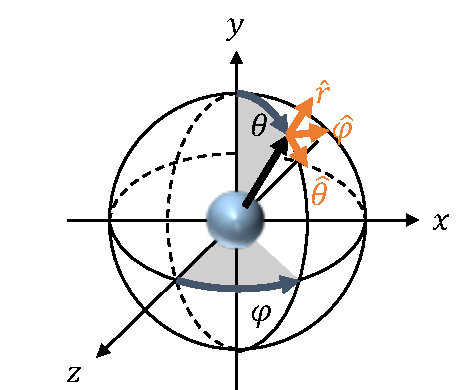
\includegraphics[scale=1.0]{/Users/taiga/Projects/lab/thesis/components/chapter2/figs/system.pdf}
        \caption{本実験の座標系}
        \label{fig:system}
    \end{figure}

マイクロスイマーのモデルとして,Squirmerモデル\cite{}を採用した.
このモデルでは,球形の粒子表面において,粒子と流体の速度差が式\eqref{eq:squirmer}で表されるようなsliding境界条件を用いる.

    \begin{equation}
        \boldsymbol{u}^\mathrm{s} = 
            \sum_{n=1}^\infty\frac{2}{n(n + 1)} B_n P_n^\prime(\cos{\theta}) \sin{\theta} \hat{\boldsymbol{\theta}}
        \label{eq:squirmer}
    \end{equation}

\noindent
ここで, 式中の$\theta, \boldsymbol{\hat{\theta}}$はFig.\ref{fig:system}のように表される角度および単位角度ベクトルである.
本研究では,$xy$平面上を$x$軸正の向きに流れるせん断流を考えたので,
Fig.\ref{fig:system}中の$\varphi$は$\pi / 2$で固定されているとした.
また,$\boldsymbol{u}^\mathrm{s}$はマイクロスイマー表面の重心に対するslide速度,
$B_n$は係数,
$P^\prime_n$は $n$次Legendre多項式の導関数である.
しかし,$n=1$の項はsquirmerの泳動速度を,
$n=2$の項はsquirmerの存在によって生じる応力を決めるが,
$n \geq 3$の項は,泳動速度,および応力に影響を与えないので,
式\eqref{eq:squirmer}は,第1,2項のみを考えることで,式\eqref{eq:squirmer2}の様に簡略化できる.

    \begin{equation}
        \boldsymbol{u}^s =
            B_1 \left( \sin{\theta} + \frac{\alpha}{2} \sin{2\theta} \right) \hat{\boldsymbol{\theta}}
        \label{eq:squirmer2}
    \end{equation}

\noindent
ここで,$B_1$はマイクロスイマーの進行速度の大きさ$(U = 2/3 B_1)$を与える.
ただし,本研究では,squirmer粒子の移動の影響を排除するために,$B_1 = 0.01$と十分に小さい値に設定した.
また,$\alpha = B_2/B_1$はその符号によりスイマーの種類を表す定数となる.
$\alpha > 0$をPuller型,$\alpha = 0$をNeutral型,$\alpha < 0$をPusher型と呼ぶ.
Puller型は,周辺流体に収縮流を生成し,Pusher型は伸長流を生成する.

    \begin{figure}[H]
        \centering
        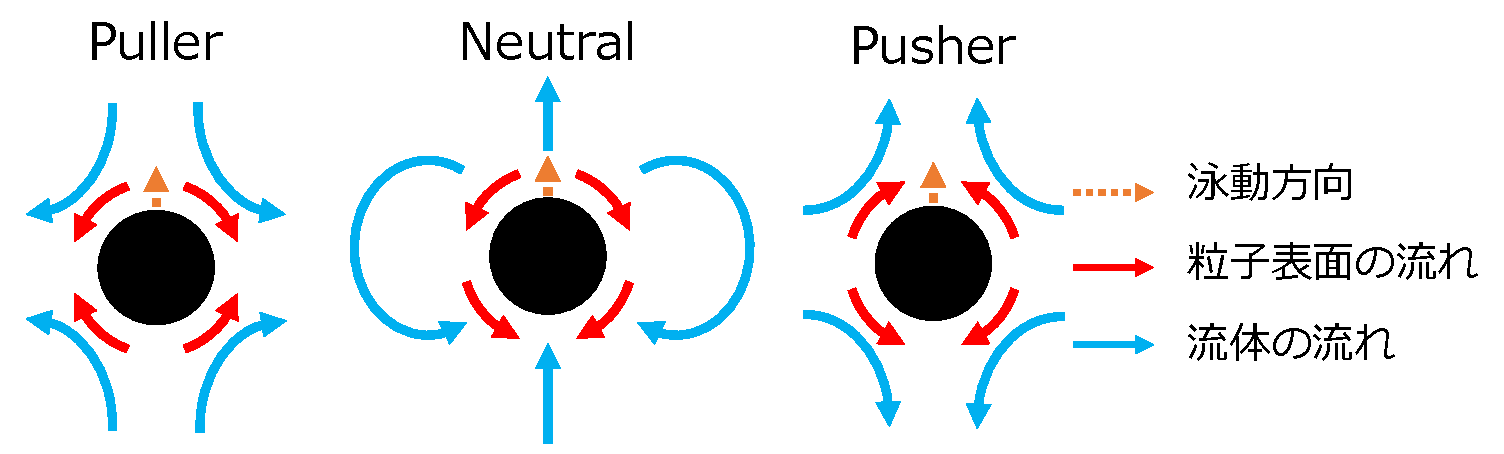
\includegraphics[scale=0.5]{/Users/taiga/Projects/lab/thesis/components/chapter2/figs/microswimmers.pdf}
        \caption{SquirmerモデルにおけるPusher型,Neutral型,Puller型の概略図}
        \label{fig:squirmermodel}
    \end{figure}

\subsection{Smoothed Profile Method}
固液二相シミュレーションにおいて,固体-液体の移動境界の取り扱いは非常に重要である.
今回のシミュレーションでは,物理量とは異なる識別関数を導入し,
仮想流体領域を考えるSmoothed Profile Method(SPM)\cite{}を用いた.
SPMでは,流体と粒子の界面にFig.\ref{fig:spm}で表されるような界面関数$\phi$を導入する.
ここで,$a$は粒子の半径,$\xi$は界面の幅を表す.
この界面関数は,流体領域で$\phi=0$,粒子領域で$\phi=1$をとり,
幅$\xi$の界面領域では滑らかに変化する連続関数である.
界面関数の導入により,境界条件を解く必要がなくなり,
計算負荷を軽減され,
以下で説明するNavier-Stokes方程式,
および運動方程式を直接数値計算によって解くことが可能となる.

    \begin{figure}[H]
        \centering
        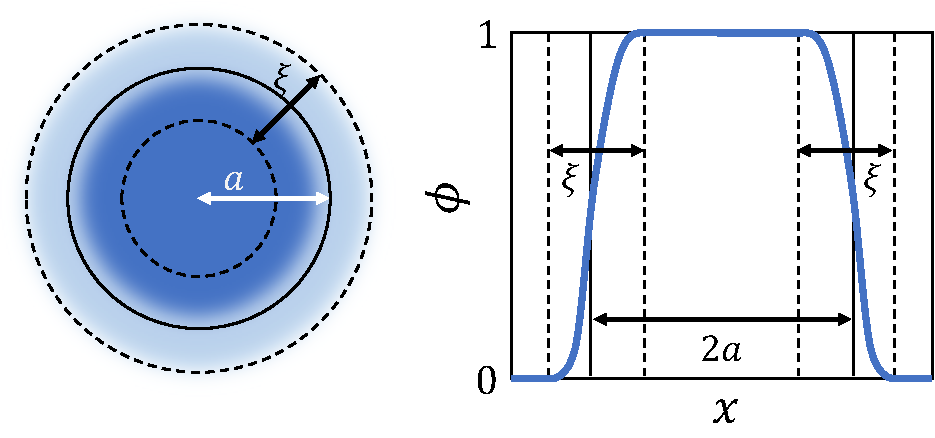
\includegraphics[scale=0.8]{/Users/taiga/Projects/lab/thesis/components/chapter2/figs/spm.pdf}
        \caption{SPMの界面関数}
        \label{fig:spm}
    \end{figure}


\subsection{支配方程式}
本研究では,流体の運動を非圧縮条件のNavier-Stokes方程式,
マイクロスイマーの運動をNewton方程式,およびEuler方程式を用いて解いた.


\subsubsection{Navier-Stokes方程式}
    \begin{align}
        \rho_\mathrm{f} (\partial _t + \boldsymbol{u} \cdot \boldsymbol{\nabla} ) \boldsymbol{u} &= 
            \boldsymbol{\nabla} \cdot \boldsymbol{\sigma} + 
            \rho_\mathrm{f} \left( \phi \boldsymbol{f}_\mathrm{p} + \boldsymbol{f}_\mathrm{sq} + \boldsymbol{f}_\mathrm{s} \right) \\
        \boldsymbol{\nabla} \cdot \boldsymbol{u} &= 0
    \end{align}

ここで,$t$は時間,
$\rho_\mathrm{f}$は流体の質量密度,
$\boldsymbol{\sigma}$は流体の応力テンソル,
$\phi \boldsymbol{f}_\mathrm{p}$は粒子の剛直性を保証する体積力,
$\boldsymbol{f}_\mathrm{sq}$は流体と粒子間の速度差を生じる力,
$\boldsymbol{f}_\mathrm{s}$はジグザグ流を生じる力である.
ジグザグ流とは,式\eqref{eq:zig_zag}のような速度プロファイルで表される流体の流れである.
この流れは,$-L_y/4 \geq y \geq L_y/4$の範囲がクエット流を表しているが,
$L_y \rightarrow \infty$を考えることで,厳密にクエット流とみなすことができる.
    \begin{equation}
        v_x(y) =
        \begin{cases}
            \dot{\gamma} \left( - y - L_y/2 \right) & (-L_y/2 < y \leq -L_y/4) \\
            \dot{\gamma} y                          & (-L_y/4 < y \leq  L_y/4) \\
            \dot{\gamma} \left( - y + L_y/2 \right) & ( L_y/4 < y \leq  L_y/2)
        \end{cases}
        \label{eq:zig_zag}
    \end{equation}

    \begin{figure}[htbp]
        \centering
        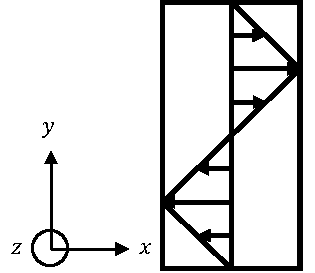
\includegraphics[scale=1.2]{/Users/taiga/Projects/lab/thesis/components/chapter2/figs/zig_zag.pdf}
        \caption{ジグザグ流の速度プロファイル}
        \label{fig:zig_zag}
    \end{figure}

\noindent
ここで,$\dot{\gamma}$はせん断速度,
$y$は$y$座標の値,
$L_y$は$y$軸方向の系の大きさである.
本研究では,せん断流を表現するためにジグザグ流を用いた.

\subsubsection{運動方程式}
\label{sec:equation_of_motion}
    \begin{align}
        \dot{\boldsymbol{R}_i} &= \boldsymbol{V}_i \\
        M_\mathrm{p} \dot{\boldsymbol{V}_i} &= \boldsymbol{F}^\mathrm{H}_i \\
        \boldsymbol{I}_\mathrm{p} \cdot \dot{\boldsymbol{\Omega}_i} &=
            \boldsymbol{N}^\mathrm{H}_i + \boldsymbol{N}^\mathrm{b.h.}_i
    \end{align}

ここで,$\boldsymbol{F}^\mathrm{H}_i$は流体から受ける力,
$\boldsymbol{N}^\mathrm{H}_i$は流体から受けるトルク,
$\boldsymbol{N}^\mathrm{b.h.}_i$はbottom heavy性によるトルクである.
$M_\mathrm{p}$は粒子の質量,
$\boldsymbol{I}_i$は慣性モーメント,
$\dot{\boldsymbol{R}_i}$は粒子の位置,
$\boldsymbol{V}_i$は粒子の速度,
$\dot{\boldsymbol{\Omega}_i}$は粒子の角速度である.
Fig.\ref{fig:bottom_heavy_fig}のように,
球の中心と粒子の重心がずれているsquirmerについて,
bottom heavy性によるトルクは式\eqref{eq:bottom_heavy}で計算される.

    \begin{equation}
        \boldsymbol{N}^\mathrm{b.h.} = \frac{4}{3} \pi a^3 \rho h \boldsymbol{e} \times \boldsymbol{g}
        \label{eq:bottom_heavy}
    \end{equation}

\noindent
ここで,$a$は粒子の半径,
$\rho$は粒子の密度,
$h$は球の中心と粒子の重心との距離,
$\boldsymbol{e}$は粒子の方向ベクトル,
$\boldsymbol{g}$は重力ベクトルである.

    \begin{figure}[htbp]
        \centering
        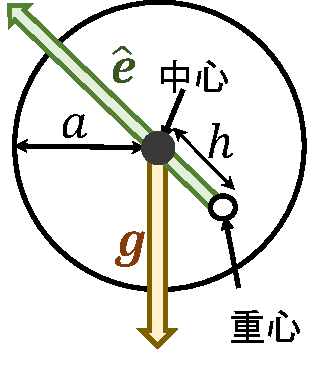
\includegraphics[scale=0.8]{/Users/taiga/Projects/lab/thesis/components/chapter2/figs/bottom_heavy.pdf}
        \caption{bottom heavy性を有するsquirmer}
        \label{fig:bottom_heavy_fig}
    \end{figure}




\end{document}
  % 方法

\newpage
\documentclass[11pt, a4j, dvipdfmx]{jarticle}
\usepackage{amsmath}
\usepackage{setspace}
\usepackage{mathtools}
\usepackage[dvipdfmx]{graphicx}  % Include figure files
% \usepackage[varg]{txfonts}
\usepackage{bm}  % bold math
\usepackage{here}
\usepackage{array}
\usepackage[T1]{fontenc}
\usepackage{etoolbox}
\usepackage[top=30truemm,bottom=30truemm,left=25truemm,right=25truemm]{geometry}  % 余白
\usepackage{comment}
\usepackage{cases}
\usepackage[version=3]{mhchem}
\usepackage{layout}
\usepackage{wrapfig}
\usepackage{indentfirst}
\usepackage{txfonts}


%\renewcommand{\indent}{\hspace*{1zw}}
\renewcommand{\abstractname}{}
\renewcommand{\figurename}{Fig.}
\renewcommand{\thefootnote}{\fnsymbol{footnote}}
\renewcommand{\thesection}{\arabic{section}}


\pagestyle{plain}
%%%%%%%%%%%%%%%%%%%%%%%%%%%%%%%%%%%%%%%%%%%%%%%%%%%%%%%%%%%%%%%%%%%%%%%%%%
\makeatletter%% プリアンブルで定義する場合は必須
\patchcmd{\maketitle}{\@fnsymbol}{\@alph}{}{}  % Footnote numbers from symbols to small letters
\long\def\@makecaption#1#2{% \@makecaption を再定義します
  \vskip\abovecaptionskip
  \iftdir\sbox\@tempboxa{#1\hskip1zw#2}%
    \else\sbox\@tempboxa{#1~ #2}  % ここの : を ~ に変更する
  \fi
  \ifdim \wd\@tempboxa >\hsize% 
    \iftdir #1\hskip1zw#2\relax\par
      \else #1~ #2\relax\par\fi  % ここの : を ~ に変更する
  \else
    \global \@minipagefalse
    \hbox to\hsize{\hfil\box\@tempboxa\hfil}  % センタリング
%   \hbox to\hsize{\box\@tempboxa\hfil}%      左詰め
%   \hbox to\hsize{\hfil\box\@tempboxa}%      右詰め
  \fi
  \vskip\belowcaptionskip}
 \DeclareRobustCommand\cite{\unskip
\@ifnextchar[{\@tempswatrue\@citex}{\@tempswafalse\@citex[]}}
 \def\@cite#1#2{$^{[\hbox{\scriptsize{#1\if@tempswa , #2\fi}]}}$}
 \def\@biblabel#1{[#1]}
\makeatother%% プリアンブルで定義する場合は必須

\setlength{\columnsep}{8  truemm}
\setlength{\linewidth}{90 truemm}


\begin{document}


\section{\large 結果と考察}


\subsection{せん断流下でのbottom heavy性を有する粒子の挙動}
\label{simulation_results}
Fig.\ref{fig:result}はシミュレーション結果を模式的に表したものである.

    \begin{figure}[htbp]
        \centering
        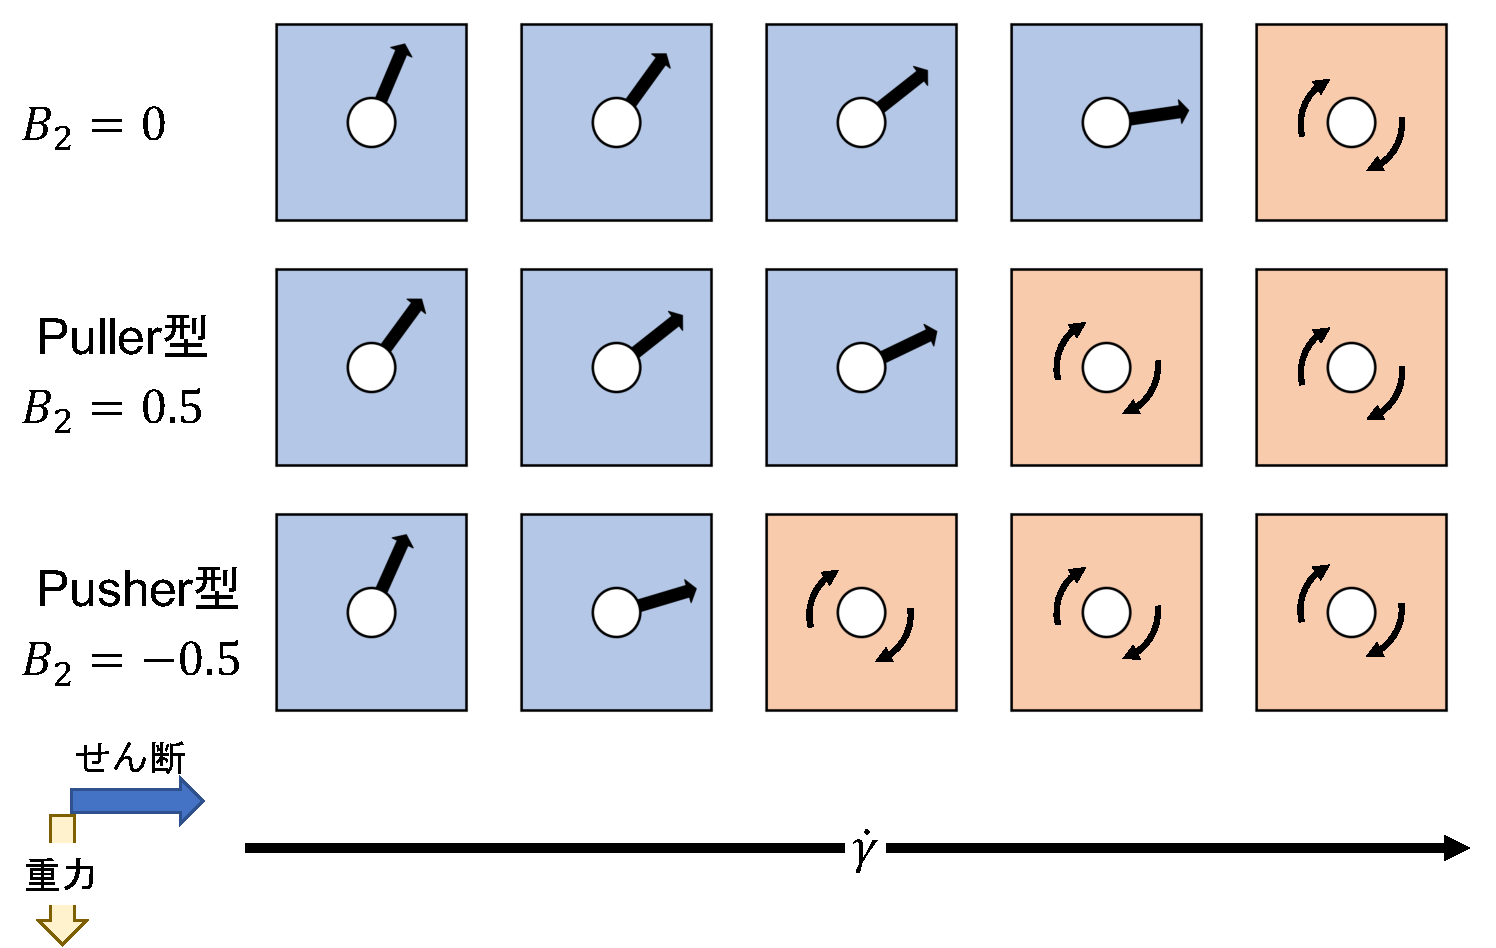
\includegraphics[scale=0.55]{/Users/taiga/Projects/lab/thesis/components/chapter4/figs/results.pdf}
        \caption{シミュレーションの模式図}
        \label{fig:result}
    \end{figure}

\noindent
上段は,通常の球形粒子にbottom heavy性を仮定したもの,
中段は,$B_2 = 0.5$のPuller型のsquirmer,
下段は,$B_2 = -0.5$のPusher型のsquirmerのシミュレーション結果である.
図中の直線の矢印は,定常せん断下での粒子の定常進行方向を表し,
曲がった矢印は粒子が定常回転していることを表す.
図の右側に行くにつれてせん断速度が大きいシミュレーションを表す.
また,左下に示したように,せん断は図の右向きに,
重力は図の下向きにかかっている.
この図より,せん断速度が小さい場合には,粒子はある進行方向に固定され,
粒子は回転せずに定常的にその方向に進むのに対し,
せん断速度が大きい場合には,定常的な回転運動を始めることが分かる.
これは,\ref{sec:rotation}で述べた予想に反しないと言うことができる.

\subsection{理論値との比較}
通常の球形粒子にbotton heavy性を仮定した場合について理論値との比較を行う.
この場合,\ref{sec:rotation}で述べたように,粒子にかかるトルクは,式\eqref{eq:sum_of_torque_z}のように表される.
    \begin{align}
        N_z &= \boldsymbol{N}^\mathrm{H}_z + \boldsymbol{N}^\mathrm{b.h.}_z \notag \\
            &= 4 \pi \mu a^3 \dot{\gamma} - \frac{4}{3} \pi \rho h g \sin \theta
        \tag{\ref{eq:sum_of_torque_z}}
    \end{align}

\noindent
このトルクはFig.\ref{fig:sum_of_torque}のように表される.

    \begin{figure}[H]
        \centering
        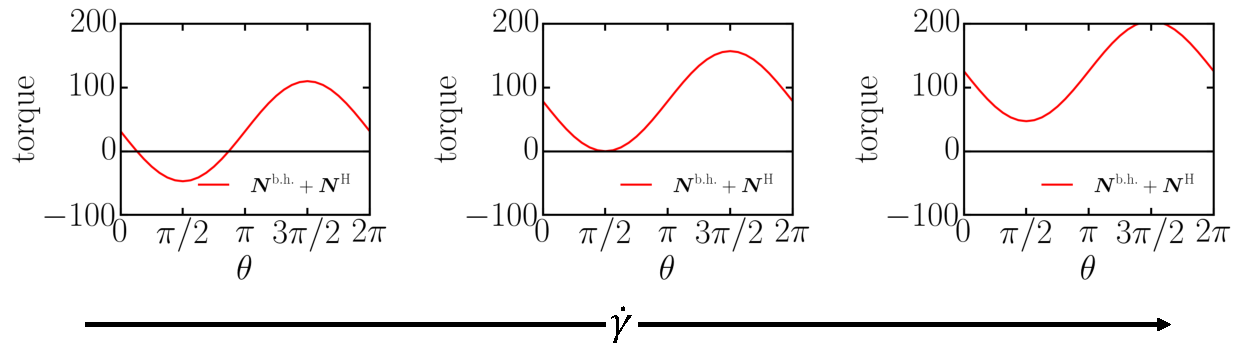
\includegraphics[scale=0.8]{/Users/taiga/Projects/lab/thesis/components/chapter4/figs/sum_of_torque.pdf}
        \caption{流体から受けるトルクとbottom heavy性によるトルクの和}
        \label{fig:sum_of_torque}
    \end{figure}

\noindent
本研究では,粒子の重心と球の中心のずれを$h = 2.5 \Delta$,重力の大きさを$g = 0.06$と設定した.
この場合,
$\dot{\gamma} < 0.05$の場合には粒子の進行方向は$0 < \theta < \pi / 2$のある角度に固定され,
$\dot{\gamma} = 0.05$の場合に,粒子の進行方向は$\theta = \pi /2$に固定され,
$\dot{\gamma} > 0.05$の場合に定常的に回転すると予想される.
Fig.\ref{fig:extracted_results}は,Fig.\ref{fig:results}の上段のシミュレーション結果を抜粋したものである.

    \begin{figure}[htbp]
        \centering
        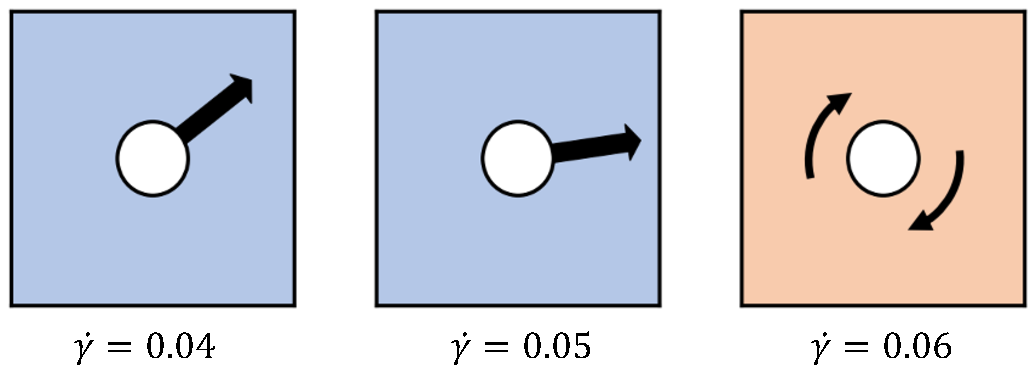
\includegraphics[scale=0.8]{/Users/taiga/Projects/lab/thesis/components/chapter4/figs/extracted_results.pdf}
        \caption{$B_2 = 0$の場合のシミュレーション模式図とそのときのせん断速度の値}
        \label{fig:extracted_results}
    \end{figure}

\noindent
この図から,シミュレーション結果が示す粒子の挙動は,理論的な式によって導かれる挙動とよく一致していることが分かる.




\end{document}
  % 予想

\newpage
\documentclass[11pt, a4j, dvipdfmx]{jarticle}
\usepackage{amsmath}
\usepackage{setspace}
\usepackage{mathtools}
\usepackage[dvipdfmx]{graphicx}  % Include figure files
% \usepackage[varg]{txfonts}
\usepackage{bm}  % bold math
\usepackage{here}
\usepackage{array}
\usepackage[T1]{fontenc}
\usepackage{etoolbox}
\usepackage[top=30truemm,bottom=30truemm,left=25truemm,right=25truemm]{geometry}  % 余白
\usepackage{comment}
\usepackage{cases}
\usepackage[version=3]{mhchem}
\usepackage{layout}
\usepackage{wrapfig}
\usepackage{indentfirst}
\usepackage{txfonts}


%\renewcommand{\indent}{\hspace*{1zw}}
\renewcommand{\abstractname}{}
\renewcommand{\figurename}{Fig.}
\renewcommand{\thefootnote}{\fnsymbol{footnote}}
\renewcommand{\thesection}{\arabic{section}}


\pagestyle{plain}
%%%%%%%%%%%%%%%%%%%%%%%%%%%%%%%%%%%%%%%%%%%%%%%%%%%%%%%%%%%%%%%%%%%%%%%%%%
\makeatletter%% プリアンブルで定義する場合は必須
\patchcmd{\maketitle}{\@fnsymbol}{\@alph}{}{}  % Footnote numbers from symbols to small letters
\long\def\@makecaption#1#2{% \@makecaption を再定義します
  \vskip\abovecaptionskip
  \iftdir\sbox\@tempboxa{#1\hskip1zw#2}%
    \else\sbox\@tempboxa{#1~ #2}  % ここの : を ~ に変更する
  \fi
  \ifdim \wd\@tempboxa >\hsize% 
    \iftdir #1\hskip1zw#2\relax\par
      \else #1~ #2\relax\par\fi  % ここの : を ~ に変更する
  \else
    \global \@minipagefalse
    \hbox to\hsize{\hfil\box\@tempboxa\hfil}  % センタリング
%   \hbox to\hsize{\box\@tempboxa\hfil}%      左詰め
%   \hbox to\hsize{\hfil\box\@tempboxa}%      右詰め
  \fi
  \vskip\belowcaptionskip}
 \DeclareRobustCommand\cite{\unskip
\@ifnextchar[{\@tempswatrue\@citex}{\@tempswafalse\@citex[]}}
 \def\@cite#1#2{$^{[\hbox{\scriptsize{#1\if@tempswa , #2\fi}]}}$}
 \def\@biblabel#1{[#1]}
\makeatother%% プリアンブルで定義する場合は必須

\setlength{\columnsep}{8  truemm}
\setlength{\linewidth}{90 truemm}


\begin{document}


\section{\large 結果と考察}


\subsection{せん断流下でのbottom heavy性を有する粒子の挙動}
\label{simulation_results}
Fig.\ref{fig:result}はシミュレーション結果を模式的に表したものである.

    \begin{figure}[htbp]
        \centering
        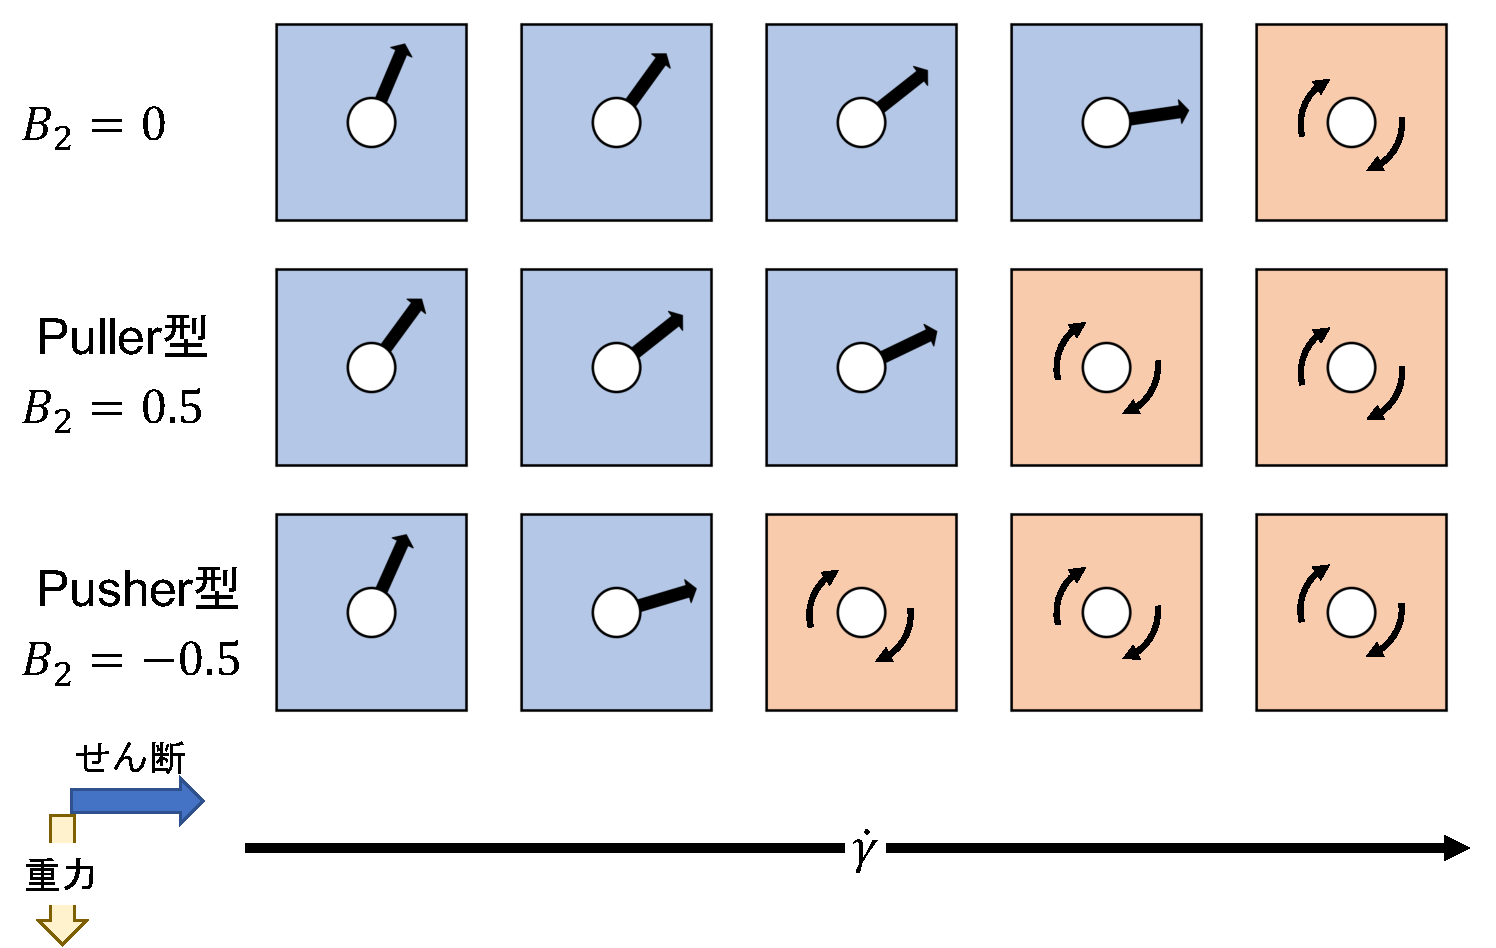
\includegraphics[scale=0.55]{/Users/taiga/Projects/lab/thesis/components/chapter4/figs/results.pdf}
        \caption{シミュレーションの模式図}
        \label{fig:result}
    \end{figure}

\noindent
上段は,通常の球形粒子にbottom heavy性を仮定したもの,
中段は,$B_2 = 0.5$のPuller型のsquirmer,
下段は,$B_2 = -0.5$のPusher型のsquirmerのシミュレーション結果である.
図中の直線の矢印は,定常せん断下での粒子の定常進行方向を表し,
曲がった矢印は粒子が定常回転していることを表す.
図の右側に行くにつれてせん断速度が大きいシミュレーションを表す.
また,左下に示したように,せん断は図の右向きに,
重力は図の下向きにかかっている.
この図より,せん断速度が小さい場合には,粒子はある進行方向に固定され,
粒子は回転せずに定常的にその方向に進むのに対し,
せん断速度が大きい場合には,定常的な回転運動を始めることが分かる.
これは,\ref{sec:rotation}で述べた予想に反しないと言うことができる.

\subsection{理論値との比較}
通常の球形粒子にbotton heavy性を仮定した場合について理論値との比較を行う.
この場合,\ref{sec:rotation}で述べたように,粒子にかかるトルクは,式\eqref{eq:sum_of_torque_z}のように表される.
    \begin{align}
        N_z &= \boldsymbol{N}^\mathrm{H}_z + \boldsymbol{N}^\mathrm{b.h.}_z \notag \\
            &= 4 \pi \mu a^3 \dot{\gamma} - \frac{4}{3} \pi \rho h g \sin \theta
        \tag{\ref{eq:sum_of_torque_z}}
    \end{align}

\noindent
このトルクはFig.\ref{fig:sum_of_torque}のように表される.

    \begin{figure}[H]
        \centering
        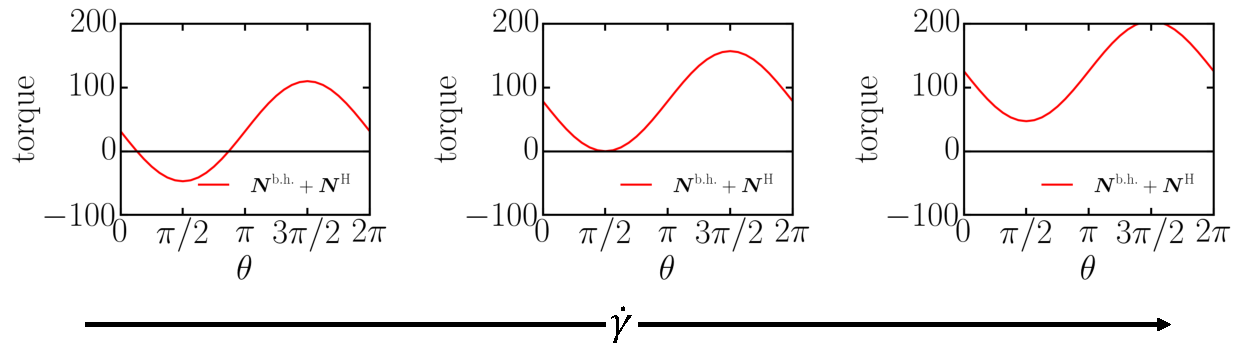
\includegraphics[scale=0.8]{/Users/taiga/Projects/lab/thesis/components/chapter4/figs/sum_of_torque.pdf}
        \caption{流体から受けるトルクとbottom heavy性によるトルクの和}
        \label{fig:sum_of_torque}
    \end{figure}

\noindent
本研究では,粒子の重心と球の中心のずれを$h = 2.5 \Delta$,重力の大きさを$g = 0.06$と設定した.
この場合,
$\dot{\gamma} < 0.05$の場合には粒子の進行方向は$0 < \theta < \pi / 2$のある角度に固定され,
$\dot{\gamma} = 0.05$の場合に,粒子の進行方向は$\theta = \pi /2$に固定され,
$\dot{\gamma} > 0.05$の場合に定常的に回転すると予想される.
Fig.\ref{fig:extracted_results}は,Fig.\ref{fig:results}の上段のシミュレーション結果を抜粋したものである.

    \begin{figure}[htbp]
        \centering
        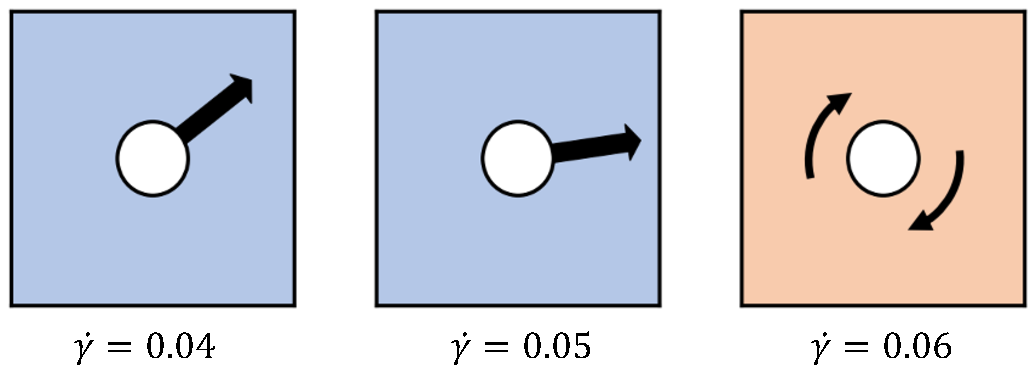
\includegraphics[scale=0.8]{/Users/taiga/Projects/lab/thesis/components/chapter4/figs/extracted_results.pdf}
        \caption{$B_2 = 0$の場合のシミュレーション模式図とそのときのせん断速度の値}
        \label{fig:extracted_results}
    \end{figure}

\noindent
この図から,シミュレーション結果が示す粒子の挙動は,理論的な式によって導かれる挙動とよく一致していることが分かる.

\subsection{有効粘度の評価}
Fig.\ref{fig:estimate_eff_viscocity}はせん断速度と有効粘度の関係を表す.

    \begin{figure}[H]
        \centering
        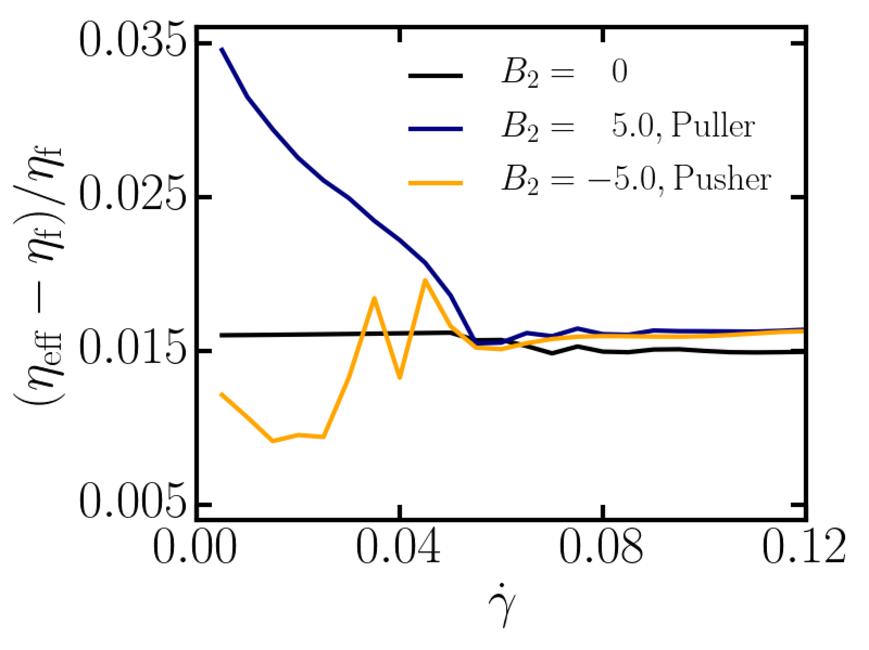
\includegraphics[scale=0.5]{/Users/taiga/Projects/lab/thesis/components/chapter4/figs/gammadot_vs_eff_viscosity.pdf}
        \caption{せん断速度と有効粘度の関係.
        黒線が通常の球形粒子にbottom heavy性を仮定したものを,
        青線が$B_1 = 5.0$のpuller型のsquirmerを,
        橙線が$B_1 = -5.0$のpusher型のsquirmerを表す.}
        \label{fig:estimate_eff_viscocity}
    \end{figure}

\noindent
このグラフから,せん断速度が小さい領域では,$B_2 > 0$のPuller型は有効粘度を大きくする方向に,
$B_2 < 0$のPusehr型は有効粘度を小さくする方向にはたらいていることが分かる.
また,せん断速度が大きい領域ではsquirmerの種類によらず,ほぼ等しい有効粘度を示していることが分かる.
Rafa\"iらによるPuller型のsquirmerであるクラミドモナスを用いたせん断速度と有効粘度の関係を検証する実験結果によると,
せん断速度が小さい領域では系の有効粘度を大きくする方向にはたらき,
せん断速度が大きい領域では,せん断速度に関わらずほぼ等しい有効粘度を示すことが分かっている\cite{effective_viscosity}.
また,MartinezaらによるPusher型のsquirmerであるE. Coli.を用いたせん断速度と有効粘度の関係を検証する実験結果によると,
同様に,せん断速度が小さい領域では系の有効粘度を小さくする方向にはたらき,
せん断速度が大きい領域では,せん断速度に関わらずほぼ等しい有効粘度を示すことが分かっている\cite{e_coli_experiment}.
これらの実験結果と今回のシミュレーション結果は定性的に一致していると言うことができる.

    \begin{figure}[htbp]
        \centering
        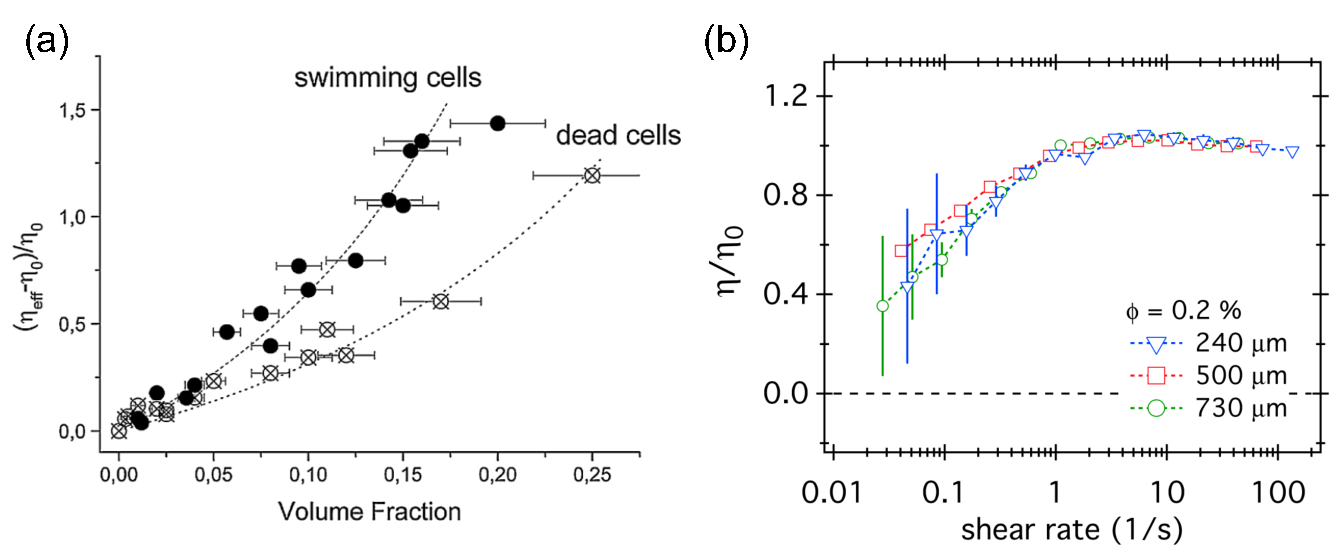
\includegraphics[scale=0.6]{/Users/taiga/Projects/lab/thesis/components/chapter4/figs/previous_effective_viscosity.pdf}
        \caption{(a)クラミドモナスのせん断速度と有効粘度の関係\cite{effective_viscosity}.
        いくつかのクラミドモナスの体積分率$\phi$における実験結果を示している.
        星形のプロットは,クラミドモナスが分散していない系の粘度を表している.
        (b)E. Coli.のせん断速度と有効粘度の関係\cite{e_coli_experiment}.
        体積分率が$\phi = 0.2 \%$の場合の実験結果を表している.
        凡例で示した値は共軸二重円筒形回転粘度計のgap sizeである.}
    \end{figure}




\end{document}
  % 結果と考察

\clearpage
\documentclass[11pt, a4j, dvipdfmx]{jarticle}
\usepackage{amsmath}
\usepackage{setspace}
\usepackage{mathtools}
\usepackage[dvipdfmx]{graphicx}  % Include figure files
% \usepackage[varg]{txfonts}
\usepackage{bm}  % bold math
\usepackage{here}
\usepackage{array}
\usepackage[T1]{fontenc}
\usepackage{etoolbox}
\usepackage[top=30truemm,bottom=30truemm,left=25truemm,right=25truemm]{geometry}  % 余白
\usepackage{comment}
\usepackage{cases}
\usepackage[version=3]{mhchem}
\usepackage{layout}
\usepackage{wrapfig}
\usepackage{indentfirst}
\usepackage{txfonts}


%\renewcommand{\indent}{\hspace*{1zw}}
\renewcommand{\abstractname}{}
\renewcommand{\figurename}{Fig.}
\renewcommand{\thefootnote}{\fnsymbol{footnote}}
\renewcommand{\thesection}{\arabic{section}}


\pagestyle{plain}
%%%%%%%%%%%%%%%%%%%%%%%%%%%%%%%%%%%%%%%%%%%%%%%%%%%%%%%%%%%%%%%%%%%%%%%%%%
\makeatletter%% プリアンブルで定義する場合は必須
\patchcmd{\maketitle}{\@fnsymbol}{\@alph}{}{}  % Footnote numbers from symbols to small letters
\long\def\@makecaption#1#2{% \@makecaption を再定義します
  \vskip\abovecaptionskip
  \iftdir\sbox\@tempboxa{#1\hskip1zw#2}%
    \else\sbox\@tempboxa{#1~ #2}  % ここの : を ~ に変更する
  \fi
  \ifdim \wd\@tempboxa >\hsize% 
    \iftdir #1\hskip1zw#2\relax\par
      \else #1~ #2\relax\par\fi  % ここの : を ~ に変更する
  \else
    \global \@minipagefalse
    \hbox to\hsize{\hfil\box\@tempboxa\hfil}  % センタリング
%   \hbox to\hsize{\box\@tempboxa\hfil}%      左詰め
%   \hbox to\hsize{\hfil\box\@tempboxa}%      右詰め
  \fi
  \vskip\belowcaptionskip}
 \DeclareRobustCommand\cite{\unskip
\@ifnextchar[{\@tempswatrue\@citex}{\@tempswafalse\@citex[]}}
 \def\@cite#1#2{$^{[\hbox{\scriptsize{#1\if@tempswa , #2\fi}]}}$}
 \def\@biblabel#1{[#1]}
\makeatother%% プリアンブルで定義する場合は必須

\setlength{\columnsep}{8  truemm}
\setlength{\linewidth}{90 truemm}


\begin{document}


\section{\large 結言}
\par

\subsection{まとめ}
本研究では,球状のsquirmerにおいて,
その重心が球の中心から後方にずれているbottom heavy性をシミュレーション上で新たに付加した後に,
bottom hevey性を付加した単体squirmerをジグザグ流を用いてせん断流を再現した系中に配置し,
その挙動を解析するシミュレーションを行った.
この性質を付加することにより,squirmerの進行方向,squirmerの重心のずれ具合,
および系にかかる重力の大きさから求まるトルクを新たに考慮することが可能となった.
Bottom heavy性を有するsquirmerの特徴的な挙動を調べるにあたり,
squirmerの存在による,系の応力および有効粘度への影響に注目した.
単体のsquirmerをせん断流下に配置すると,
せん断流の大きさに比例するトルクを受ける.
また,bottom heavy性によるトルクの大きさはsquirmerの進行方向に依存するサイン関数となる.
そのため,bottom heavy性によるトルクの最大の絶対値と流体から受けるトルクの大きさが同じ値となるせん断速度$\dot{\gamma}_c$が存在し,
その値との大小関係からsquirmerの回転運動の有無を予想できる.
せん断速度が$\dot{\gamma}_c$より小さい場合には,
bottom heavy性によるトルクが支配的となるため,
squirmerの進行方向は$0 \leq \theta < 2 \pi$の範囲内に固定され,回転運動をしないことが予想される.
また,せん断速度が$\dot{\gamma}_c$に等しい場合には,
bottom heavy性によるトルクが最小値をとる$\theta = \pi / 2$に固定され,
回転運動をしないことが予想される.
さらに,せん断速度が$\dot{\gamma}_c$より大きい場合には,
流体から受けるトルクが支配的となり,
squirmerは定常的に回転運動をすることが予想される.
Squirmerが存在することで生じる応力は,
squirmerの進行方向に依存した,サイン関数とコサイン関数を掛け合わせた関数となる.
そのため,squirmerの進行方向が固定される場合には,
squirmerの存在による応力が生じ,系の応力に影響を与えることが予想される.
一方,squirmerが定常的に等角速度で回転している場合には,
squirmerの存在による応力の時間平均をとるとプラスとマイナスが打ち消し合い,
系の応力には影響を与えないことが予想される.
さらに,有効粘度は,系の応力をせん断速度で割ることで求めることができるため,
系の応力への影響と同じ傾向が有効粘度の値にも見られることが予想される.
シミュレーションを行った結果,
球形粒子にbottom heavy性を仮定したものについて,
$\dot{\gamma}_c$の値,
およびせん断速度が$\dot{\gamma}_c$よりも小さい場合に固定される,squirmerの進行方向の角度が
シミュレーション結果と理論的に求まる値とで十分に一致していることを確認した.
さらに,せん断速度が$\dot{\gamma}_c$より小さい領域で,
Puller型の場合は,有効粘度を大きくする方向に,
Pusher型の場合は,有効粘度を小さくする方向にはたらくことが確認できた.
また,せん断速度が$\dot{\gamma}_c$より大きい領域では,
squirmerの種類によらず,ほぼ等しい有効粘度を示すことが確認できた.
この傾向は,Puller型であるクラミドモナス
およびPusher型であるE. Coli.を用いた実験により得られた結果と定性的に一致していることを確認した.

\subsection{今後の課題}
本研究では,マイクロスイマーの移動によるシミュレーションへの影響を排除するために
$B_1$の値を十分に小さな値に設定したが,
より現実のマイクロスイマーの挙動に近づけるためには,
それらの影響を考慮したシミュレーションを行う必要がある.
また,有効粘度の解析結果は,定性的な考察であるため,
定量的に解析を行いシミュレーションの妥当性を評価することが課題の1つとして挙げられる.
さらに,本研究では,マイクロスイマー単体が存在する系についてシミュレーションおよび解析を行ったが,
マイクロスイマーが多数分散する系について同様のシミュレーションを行い,
特徴的な挙動が見られるかを検証することも課題として挙げられる.



\end{document}
  % 結言

\newpage
\documentclass[11pt, a4j, dvipdfmx]{jarticle}
\usepackage{amsmath}
\usepackage{setspace}
\usepackage{mathtools}
\usepackage[dvipdfmx]{graphicx}  % Include figure files
% \usepackage[varg]{txfonts}
\usepackage{bm}  % bold math
\usepackage{here}
\usepackage{array}
\usepackage[T1]{fontenc}
\usepackage{etoolbox}
\usepackage[top=30truemm,bottom=30truemm,left=25truemm,right=25truemm]{geometry}  % 余白
\usepackage{comment}
\usepackage{cases}
\usepackage[version=3]{mhchem}
\usepackage{layout}
\usepackage{wrapfig}
\usepackage{indentfirst}
\usepackage{txfonts}


%\renewcommand{\indent}{\hspace*{1zw}}
\renewcommand{\abstractname}{}
\renewcommand{\figurename}{Fig.}
\renewcommand{\thefootnote}{\fnsymbol{footnote}}
\renewcommand{\thesection}{\arabic{section}}


\pagestyle{plain}
%%%%%%%%%%%%%%%%%%%%%%%%%%%%%%%%%%%%%%%%%%%%%%%%%%%%%%%%%%%%%%%%%%%%%%%%%%
\makeatletter%% プリアンブルで定義する場合は必須
\patchcmd{\maketitle}{\@fnsymbol}{\@alph}{}{}  % Footnote numbers from symbols to small letters
\long\def\@makecaption#1#2{% \@makecaption を再定義します
  \vskip\abovecaptionskip
  \iftdir\sbox\@tempboxa{#1\hskip1zw#2}%
    \else\sbox\@tempboxa{#1~ #2}  % ここの : を ~ に変更する
  \fi
  \ifdim \wd\@tempboxa >\hsize% 
    \iftdir #1\hskip1zw#2\relax\par
      \else #1~ #2\relax\par\fi  % ここの : を ~ に変更する
  \else
    \global \@minipagefalse
    \hbox to\hsize{\hfil\box\@tempboxa\hfil}  % センタリング
%   \hbox to\hsize{\box\@tempboxa\hfil}%      左詰め
%   \hbox to\hsize{\hfil\box\@tempboxa}%      右詰め
  \fi
  \vskip\belowcaptionskip}
 \DeclareRobustCommand\cite{\unskip
\@ifnextchar[{\@tempswatrue\@citex}{\@tempswafalse\@citex[]}}
 \def\@cite#1#2{$^{[\hbox{\scriptsize{#1\if@tempswa , #2\fi}]}}$}
 \def\@biblabel#1{[#1]}
\makeatother%% プリアンブルで定義する場合は必須

\setlength{\columnsep}{8  truemm}
\setlength{\linewidth}{90 truemm}


\begin{document}

\addcontentsline{toc}{section}{謝辞}
\section*{謝辞}
本研究をご指導いただいた山本量一教授にまず心より御礼申し上げます.
コロイド粒子分散系について基礎的な知識もなかった私に何度も丁寧にご指導いただき,多くのことを学べました.
先生のご指導なしでは,私の拙い研究が卒業論文という形にまとまらなかったと思います.
ゼミや普段の研究生活でご助言いただいた谷口貴志准教授,John Molina助教に心よりお礼申し上げます.
鋭い考察で研究について指導してくださったD2の佐藤さん,M2の小栗さん,笹倉さん,馬場さん,松田さん,土岸さん,スライドの体裁や発表について丁寧に指導してくださったM1の瀬領さん,玉造さん,濱田さん,山口さん,養田さん,張さんに心よりお礼申し上げます.
最後に,同輩たちはとても優秀で刺激を受ける機会が多く,充実した研究生活が送れました.1講座の皆様,本当にありがとうございました.

\end{document}
  % 謝辞

\clearpage
\documentclass[12pt, a4j, dvipdfmx]{jarticle}
\usepackage{amsmath}
\usepackage{setspace}
\usepackage{mathtools}
\usepackage[dvipdfmx]{graphicx}  % Include figure files
% \usepackage[varg]{txfonts}
\usepackage{bm}  % bold math
\usepackage{here}
\usepackage{array}
\usepackage[T1]{fontenc}
\usepackage{etoolbox}
\usepackage[top=30truemm,bottom=30truemm,left=25truemm,right=25truemm]{geometry}  % 余白
\usepackage{comment}
\usepackage{cases}
\usepackage[version=3]{mhchem}
\usepackage{layout}
\usepackage{wrapfig}
\usepackage{indentfirst}
\usepackage{txfonts}


%\renewcommand{\indent}{\hspace*{1zw}}
\renewcommand{\abstractname}{}
\renewcommand{\figurename}{Fig.}
\renewcommand{\thefootnote}{\fnsymbol{footnote}}
\renewcommand{\thesection}{\arabic{section}}


\pagestyle{plain}
%%%%%%%%%%%%%%%%%%%%%%%%%%%%%%%%%%%%%%%%%%%%%%%%%%%%%%%%%%%%%%%%%%%%%%%%%%
\makeatletter%% プリアンブルで定義する場合は必須
\patchcmd{\maketitle}{\@fnsymbol}{\@alph}{}{}  % Footnote numbers from symbols to small letters
\long\def\@makecaption#1#2{% \@makecaption を再定義します
  \vskip\abovecaptionskip
  \iftdir\sbox\@tempboxa{#1\hskip1zw#2}%
    \else\sbox\@tempboxa{#1~ #2}  % ここの : を ~ に変更する
  \fi
  \ifdim \wd\@tempboxa >\hsize% 
    \iftdir #1\hskip1zw#2\relax\par
      \else #1~ #2\relax\par\fi  % ここの : を ~ に変更する
  \else
    \global \@minipagefalse
    \hbox to\hsize{\hfil\box\@tempboxa\hfil}  % センタリング
%   \hbox to\hsize{\box\@tempboxa\hfil}%      左詰め
%   \hbox to\hsize{\hfil\box\@tempboxa}%      右詰め
  \fi
  \vskip\belowcaptionskip}
 \DeclareRobustCommand\cite{\unskip
\@ifnextchar[{\@tempswatrue\@citex}{\@tempswafalse\@citex[]}}
 \def\@cite#1#2{$^{[\hbox{\scriptsize{#1\if@tempswa , #2\fi}]}}$}
 \def\@biblabel#1{[#1]}
\makeatother%% プリアンブルで定義する場合は必須

\setlength{\columnsep}{8  truemm}
\setlength{\linewidth}{90 truemm}


\begin{document}


\addcontentsline{toc}{section}{参考文献}
\renewcommand{\refname}{参考文献}
\begin{thebibliography}{99}
%
\bibitem{pedestrian}
D. Helbing, \textit{et al.}, \textit{Transport. Sci.}, \textbf{39}, 1(2005)\\
%
\bibitem{Teun}
Teun Vissers, \textit{et al.}, \textit{Soft Matter}, \textbf{7}, 2352(2011)\\
%
\bibitem{spm}
Yasuya Nakayama and Ryoichi Yamamoto, \textit{Phys. Rev. E}, \textbf{71}, 036707(2005)\\
%
\bibitem{Henry}
Hiroyuki Ohshima, \textit{J. Colloid Interface Sci.}, \textbf{180}, 299(1996)\\
\vspace{-8truemm}\\
\end{thebibliography}


\end{document}
  % 参考文献

% \newpage
% \documentclass[12pt, a4j, dvipdfmx]{jarticle}
\usepackage{amsmath}
\usepackage{setspace}
\usepackage{mathtools}
\usepackage[dvipdfmx]{graphicx}  % Include figure files
% \usepackage[varg]{txfonts}
\usepackage{bm}  % bold math
\usepackage{here}
\usepackage{array}
\usepackage[T1]{fontenc}
\usepackage{etoolbox}
\usepackage[top=30truemm,bottom=30truemm,left=25truemm,right=25truemm]{geometry}  % 余白
\usepackage{comment}
\usepackage{cases}
\usepackage[version=3]{mhchem}
\usepackage{layout}
\usepackage{wrapfig}
\usepackage{indentfirst}
\usepackage{txfonts}


%\renewcommand{\indent}{\hspace*{1zw}}
\renewcommand{\abstractname}{}
\renewcommand{\figurename}{Fig.}
\renewcommand{\thefootnote}{\fnsymbol{footnote}}
\renewcommand{\thesection}{\arabic{section}}


\pagestyle{plain}
%%%%%%%%%%%%%%%%%%%%%%%%%%%%%%%%%%%%%%%%%%%%%%%%%%%%%%%%%%%%%%%%%%%%%%%%%%
\makeatletter%% プリアンブルで定義する場合は必須
\patchcmd{\maketitle}{\@fnsymbol}{\@alph}{}{}  % Footnote numbers from symbols to small letters
\long\def\@makecaption#1#2{% \@makecaption を再定義します
  \vskip\abovecaptionskip
  \iftdir\sbox\@tempboxa{#1\hskip1zw#2}%
    \else\sbox\@tempboxa{#1~ #2}  % ここの : を ~ に変更する
  \fi
  \ifdim \wd\@tempboxa >\hsize% 
    \iftdir #1\hskip1zw#2\relax\par
      \else #1~ #2\relax\par\fi  % ここの : を ~ に変更する
  \else
    \global \@minipagefalse
    \hbox to\hsize{\hfil\box\@tempboxa\hfil}  % センタリング
%   \hbox to\hsize{\box\@tempboxa\hfil}%      左詰め
%   \hbox to\hsize{\hfil\box\@tempboxa}%      右詰め
  \fi
  \vskip\belowcaptionskip}
 \DeclareRobustCommand\cite{\unskip
\@ifnextchar[{\@tempswatrue\@citex}{\@tempswafalse\@citex[]}}
 \def\@cite#1#2{$^{[\hbox{\scriptsize{#1\if@tempswa , #2\fi}]}}$}
 \def\@biblabel#1{[#1]}
\makeatother%% プリアンブルで定義する場合は必須

\setlength{\columnsep}{8  truemm}
\setlength{\linewidth}{90 truemm}


\begin{document}


\addcontentsline{toc}{section}{Appendix}
\section*{Appendix}
\setcounter{subsection}{0}
\def\thesubsection{\Alph{subsection}}
\subsection{パラメーター一覧}

\begin{table}[H]
  \centering
  \begin{tabular}{lcr}
    \hline
    記号  & パラメーター \\
    \hline \hline
    $\Delta$ &格子幅\\
    $a$  & 粒子半径\\
    $d$  & 粒子径\\
    $\lambda_B$  & ビエルム長\\
    $e$ &  電気素量\\
    $k_\textrm{B}$  & ボルツマン定数\\
    $T$ &絶対温度\\
    $E$  & 電場強度\\
    $\epsilon$  & 誘電率\\
    $\eta$  & 溶媒の粘度\\
    $\rho$  & 溶媒の密度\\
    $D_\alpha$ &  拡散係数\\
    $z_\alpha$ &  $\alpha$種のイオン価数\\
    $\Psi$  & 静電ポテンシャル\\
    $\kappa^{-1}$  & デバイ長さ\\
    $\phi$  & 界面関数\\
    $\xi$  & 界面幅\\
    $\boldsymbol{f_{\textrm{p}}}$  & 粒子の剛体性を保証する力\\
    $\boldsymbol{n}$ & 単位ベクトル\\
    $\boldsymbol{I}$ &  単位テンソル\\
    $C_\alpha$  & イオン密度\\
    $C_\alpha^*$  & 補助イオン密度\\
    $\mu_\alpha$  & 化学ポテンシャル\\
    $M_{\textrm{p}}$ &  粒子質量\\
    $\boldsymbol{V_i}$  & 粒子$i$の速度\\
    $\boldsymbol{F_i^{\textrm{H}}}$ &  粒子$i$に働く流体からの力\\
    $\boldsymbol{F_i^{\textrm{C}}}$  & 粒子$i$に働く相互作用力\\
    $\boldsymbol{R_i}$  & 粒子$i$の位置\\
    $\boldsymbol{I_{\textrm{p}}}$ &  粒子の慣性モーメント\\
    $\boldsymbol{\Omega_i}$ &  粒子$i$の角速度\\
    $\boldsymbol{N_i^{\textrm{H}}}$  & 粒子$i$のトルク\\
    \hline
  \end{tabular}
\end{table}


\end{document}
  % Appendix

\end{document}
